% Options for packages loaded elsewhere
\PassOptionsToPackage{unicode}{hyperref}
\PassOptionsToPackage{hyphens}{url}
\PassOptionsToPackage{dvipsnames,svgnames,x11names}{xcolor}
%
\documentclass[
  letterpaper,
  DIV=11,
  numbers=noendperiod]{scrartcl}

\usepackage{amsmath,amssymb}
\usepackage{iftex}
\ifPDFTeX
  \usepackage[T1]{fontenc}
  \usepackage[utf8]{inputenc}
  \usepackage{textcomp} % provide euro and other symbols
\else % if luatex or xetex
  \usepackage{unicode-math}
  \defaultfontfeatures{Scale=MatchLowercase}
  \defaultfontfeatures[\rmfamily]{Ligatures=TeX,Scale=1}
\fi
\usepackage{lmodern}
\ifPDFTeX\else  
    % xetex/luatex font selection
\fi
% Use upquote if available, for straight quotes in verbatim environments
\IfFileExists{upquote.sty}{\usepackage{upquote}}{}
\IfFileExists{microtype.sty}{% use microtype if available
  \usepackage[]{microtype}
  \UseMicrotypeSet[protrusion]{basicmath} % disable protrusion for tt fonts
}{}
\makeatletter
\@ifundefined{KOMAClassName}{% if non-KOMA class
  \IfFileExists{parskip.sty}{%
    \usepackage{parskip}
  }{% else
    \setlength{\parindent}{0pt}
    \setlength{\parskip}{6pt plus 2pt minus 1pt}}
}{% if KOMA class
  \KOMAoptions{parskip=half}}
\makeatother
\usepackage{xcolor}
\setlength{\emergencystretch}{3em} % prevent overfull lines
\setcounter{secnumdepth}{-\maxdimen} % remove section numbering
% Make \paragraph and \subparagraph free-standing
\makeatletter
\ifx\paragraph\undefined\else
  \let\oldparagraph\paragraph
  \renewcommand{\paragraph}{
    \@ifstar
      \xxxParagraphStar
      \xxxParagraphNoStar
  }
  \newcommand{\xxxParagraphStar}[1]{\oldparagraph*{#1}\mbox{}}
  \newcommand{\xxxParagraphNoStar}[1]{\oldparagraph{#1}\mbox{}}
\fi
\ifx\subparagraph\undefined\else
  \let\oldsubparagraph\subparagraph
  \renewcommand{\subparagraph}{
    \@ifstar
      \xxxSubParagraphStar
      \xxxSubParagraphNoStar
  }
  \newcommand{\xxxSubParagraphStar}[1]{\oldsubparagraph*{#1}\mbox{}}
  \newcommand{\xxxSubParagraphNoStar}[1]{\oldsubparagraph{#1}\mbox{}}
\fi
\makeatother

\usepackage{color}
\usepackage{fancyvrb}
\newcommand{\VerbBar}{|}
\newcommand{\VERB}{\Verb[commandchars=\\\{\}]}
\DefineVerbatimEnvironment{Highlighting}{Verbatim}{commandchars=\\\{\}}
% Add ',fontsize=\small' for more characters per line
\usepackage{framed}
\definecolor{shadecolor}{RGB}{241,243,245}
\newenvironment{Shaded}{\begin{snugshade}}{\end{snugshade}}
\newcommand{\AlertTok}[1]{\textcolor[rgb]{0.68,0.00,0.00}{#1}}
\newcommand{\AnnotationTok}[1]{\textcolor[rgb]{0.37,0.37,0.37}{#1}}
\newcommand{\AttributeTok}[1]{\textcolor[rgb]{0.40,0.45,0.13}{#1}}
\newcommand{\BaseNTok}[1]{\textcolor[rgb]{0.68,0.00,0.00}{#1}}
\newcommand{\BuiltInTok}[1]{\textcolor[rgb]{0.00,0.23,0.31}{#1}}
\newcommand{\CharTok}[1]{\textcolor[rgb]{0.13,0.47,0.30}{#1}}
\newcommand{\CommentTok}[1]{\textcolor[rgb]{0.37,0.37,0.37}{#1}}
\newcommand{\CommentVarTok}[1]{\textcolor[rgb]{0.37,0.37,0.37}{\textit{#1}}}
\newcommand{\ConstantTok}[1]{\textcolor[rgb]{0.56,0.35,0.01}{#1}}
\newcommand{\ControlFlowTok}[1]{\textcolor[rgb]{0.00,0.23,0.31}{\textbf{#1}}}
\newcommand{\DataTypeTok}[1]{\textcolor[rgb]{0.68,0.00,0.00}{#1}}
\newcommand{\DecValTok}[1]{\textcolor[rgb]{0.68,0.00,0.00}{#1}}
\newcommand{\DocumentationTok}[1]{\textcolor[rgb]{0.37,0.37,0.37}{\textit{#1}}}
\newcommand{\ErrorTok}[1]{\textcolor[rgb]{0.68,0.00,0.00}{#1}}
\newcommand{\ExtensionTok}[1]{\textcolor[rgb]{0.00,0.23,0.31}{#1}}
\newcommand{\FloatTok}[1]{\textcolor[rgb]{0.68,0.00,0.00}{#1}}
\newcommand{\FunctionTok}[1]{\textcolor[rgb]{0.28,0.35,0.67}{#1}}
\newcommand{\ImportTok}[1]{\textcolor[rgb]{0.00,0.46,0.62}{#1}}
\newcommand{\InformationTok}[1]{\textcolor[rgb]{0.37,0.37,0.37}{#1}}
\newcommand{\KeywordTok}[1]{\textcolor[rgb]{0.00,0.23,0.31}{\textbf{#1}}}
\newcommand{\NormalTok}[1]{\textcolor[rgb]{0.00,0.23,0.31}{#1}}
\newcommand{\OperatorTok}[1]{\textcolor[rgb]{0.37,0.37,0.37}{#1}}
\newcommand{\OtherTok}[1]{\textcolor[rgb]{0.00,0.23,0.31}{#1}}
\newcommand{\PreprocessorTok}[1]{\textcolor[rgb]{0.68,0.00,0.00}{#1}}
\newcommand{\RegionMarkerTok}[1]{\textcolor[rgb]{0.00,0.23,0.31}{#1}}
\newcommand{\SpecialCharTok}[1]{\textcolor[rgb]{0.37,0.37,0.37}{#1}}
\newcommand{\SpecialStringTok}[1]{\textcolor[rgb]{0.13,0.47,0.30}{#1}}
\newcommand{\StringTok}[1]{\textcolor[rgb]{0.13,0.47,0.30}{#1}}
\newcommand{\VariableTok}[1]{\textcolor[rgb]{0.07,0.07,0.07}{#1}}
\newcommand{\VerbatimStringTok}[1]{\textcolor[rgb]{0.13,0.47,0.30}{#1}}
\newcommand{\WarningTok}[1]{\textcolor[rgb]{0.37,0.37,0.37}{\textit{#1}}}

\providecommand{\tightlist}{%
  \setlength{\itemsep}{0pt}\setlength{\parskip}{0pt}}\usepackage{longtable,booktabs,array}
\usepackage{calc} % for calculating minipage widths
% Correct order of tables after \paragraph or \subparagraph
\usepackage{etoolbox}
\makeatletter
\patchcmd\longtable{\par}{\if@noskipsec\mbox{}\fi\par}{}{}
\makeatother
% Allow footnotes in longtable head/foot
\IfFileExists{footnotehyper.sty}{\usepackage{footnotehyper}}{\usepackage{footnote}}
\makesavenoteenv{longtable}
\usepackage{graphicx}
\makeatletter
\newsavebox\pandoc@box
\newcommand*\pandocbounded[1]{% scales image to fit in text height/width
  \sbox\pandoc@box{#1}%
  \Gscale@div\@tempa{\textheight}{\dimexpr\ht\pandoc@box+\dp\pandoc@box\relax}%
  \Gscale@div\@tempb{\linewidth}{\wd\pandoc@box}%
  \ifdim\@tempb\p@<\@tempa\p@\let\@tempa\@tempb\fi% select the smaller of both
  \ifdim\@tempa\p@<\p@\scalebox{\@tempa}{\usebox\pandoc@box}%
  \else\usebox{\pandoc@box}%
  \fi%
}
% Set default figure placement to htbp
\def\fps@figure{htbp}
\makeatother

\KOMAoption{captions}{tableheading}
\makeatletter
\@ifpackageloaded{caption}{}{\usepackage{caption}}
\AtBeginDocument{%
\ifdefined\contentsname
  \renewcommand*\contentsname{Table of contents}
\else
  \newcommand\contentsname{Table of contents}
\fi
\ifdefined\listfigurename
  \renewcommand*\listfigurename{List of Figures}
\else
  \newcommand\listfigurename{List of Figures}
\fi
\ifdefined\listtablename
  \renewcommand*\listtablename{List of Tables}
\else
  \newcommand\listtablename{List of Tables}
\fi
\ifdefined\figurename
  \renewcommand*\figurename{Figure}
\else
  \newcommand\figurename{Figure}
\fi
\ifdefined\tablename
  \renewcommand*\tablename{Table}
\else
  \newcommand\tablename{Table}
\fi
}
\@ifpackageloaded{float}{}{\usepackage{float}}
\floatstyle{ruled}
\@ifundefined{c@chapter}{\newfloat{codelisting}{h}{lop}}{\newfloat{codelisting}{h}{lop}[chapter]}
\floatname{codelisting}{Listing}
\newcommand*\listoflistings{\listof{codelisting}{List of Listings}}
\makeatother
\makeatletter
\makeatother
\makeatletter
\@ifpackageloaded{caption}{}{\usepackage{caption}}
\@ifpackageloaded{subcaption}{}{\usepackage{subcaption}}
\makeatother

\usepackage{bookmark}

\IfFileExists{xurl.sty}{\usepackage{xurl}}{} % add URL line breaks if available
\urlstyle{same} % disable monospaced font for URLs
\hypersetup{
  pdftitle={DATA 609 - Homework 6: Applications to Stats and Machine Learning},
  pdfauthor={Eddie Xu},
  colorlinks=true,
  linkcolor={blue},
  filecolor={Maroon},
  citecolor={Blue},
  urlcolor={Blue},
  pdfcreator={LaTeX via pandoc}}


\title{DATA 609 - Homework 6: Applications to Stats and Machine
Learning}
\author{Eddie Xu}
\date{}

\begin{document}
\maketitle


\subsection{Instructions}\label{instructions}

Please submit a .qmd file along with a rendered pdf to the Brightspace
page for this assignment. You may use whatever language you like within
your qmd file, I recommend python, julia, or R.

\subsection{Problem 1: Multi-Label Support Vector Machine (CVX
Additional Exercises
6.18)}\label{problem-1-multi-label-support-vector-machine-cvx-additional-exercises-6.18}

The basic SVM described in chapter 8 of the book is used for
classification of data with two labels. In this problem we explore an
extension of SVM that can be used to carry out classification of data
with more than two labels. Our data consists of pairs:

\[
(\mathbf{x}_i , y_i ) \in \mathbf{R}^n \times \{1, \dots , K\},\, i = 1, \dots , m
\]

where \(\mathbf{x}_i\) is the feature vector and \(y_i\) is the label of
the \(i\)th data point. (So the labels can take the values
\(1, \dots , K\).)

Our classifier will use \(K\) affine functions,
\(f_k(\mathbf{x}) = \mathbf{a}^T_k \mathbf{x} + \mathbf{b}_k\),
\(k = 1, . . . , K\), which we also collect into affine function from
\(\mathbb{R}^n\) into \(\mathbb{R}^K\) as
\(f(\mathbf{x}) = A\mathbf{x} + \mathbf{b}\). (Therows of \(A\) are
\(\mathbf{a}^T_k\) .) Given the feature vector \(\mathbf{x}\), our model
predicts the label \(\hat{y} = \mathrm{argmax}_k f_k (\mathbf{x})\),
i.e.~the predicted label is given by the index of the largest value of
the \(f_k\) functions evaluated at the data point.

We assume that exact ties never occur, or if they do, an arbitrary
choice can be made. Note that if a multiple of 1 is added to
\(\mathbf{b}\), the classifier does not change. Thus, without loss of
generality, we can assume that \(\mathbf{1}^T \mathbf{b} = 0\).

To correctly classify all the data examples perfectly, we would need
\(f_{y_i} (\mathbf{x}_i ) > \mathrm{max}_{k\neq y_i} f_k (\mathbf{x}_i )\)
for all \(i\). This set of inequalities in \(a_k\) and \(b_k\), are
feasible if and only if the set of inequalities
\(f_{y_i} (\mathbf{x}_i ) \geq 1 + \mathrm{max}_{k\neq y_i} f_k (\mathbf{x}_i )\)
are feasible. This motivates the loss function:

\[
L(A, \mathbf{b}) = \sum_{i=1}^m\left(1 + \mathrm{max}_{k \neq y_i}f_k(\mathbf{x}_i) - f_{y_i}(\mathbf{x}_i)  \right)_+
\]

where \((u)_+ = \mathrm{max}\{u, 0\}\). The multi-label SVM chooses
\(A\) and \(\mathbf{b}\) to minimize \(L(A, b) + \mu\|A\|_F^2,\) subject
to \(\mathbf{1}^T \mathbf{b} = 0\), where \(\mu > 0\) is a
regularization parameter. (Several variations on this are possible, such
as regularizing b as well, or replacing the Frobenius norm squared with
the sum of norms of the columns of A.). The Frobenius norm is a
generalization of the \(2\)-norm from vectors to matrices, it is defined
as \(\|A\|_F = \left(\sum_{ij} A_{ij}^2\right)^{1/2}\) and implemented
in \texttt{CVX} using
\texttt{norm(A,\textquotesingle{}fro\textquotesingle{})}.

\begin{enumerate}
\def\labelenumi{(\alph{enumi})}
\item
  Show how to find \(A\) and \(\mathbf{b}\) using convex optimization.
  Be sure to justify any changes of variables or reformulation (if
  needed), and convexity of the objective and constraints in your
  formulation.
\item
  Carry out multi-label SVM on the data given in
  \href{https://github.com/georgehagstrom/DATA609Spring2025/blob/main/website/assignments/labs/labData/multi_label_svm_data.csv}{multi\_label\_svm\_data.csv}.
\end{enumerate}

Use the data given in \(\mathbf{X}\) and \(y\) to fit the SVM model, for
a range of values of \(\mu\). Use the data given in
\href{https://github.com/georgehagstrom/DATA609Spring2025/blob/main/website/assignments/labs/labData/multi_label_svm_test.csv}{multi\_label\_svm\_test.csv}
to test the SVM models. Plot the test set classification error rate
(i.e., the fraction of data examples in the test set for which
\(\hat{y} \neq y\)) versus \(\mu\).

You don't need to try more than 10 or 20 values of \(\mu\), and we
suggest choosing them uniformly on a \texttt{log} scale, from (say)
\(10^{−2}\) to \(10^2\).

\subsubsection{Problem 1(a) Solution}\label{problem-1a-solution}

The problem can be solved using convex optimization because the
constraint is affline, therfore it is convex. The hinge loss term is
convex and the regulation term, robenius norm squared term is also
convex in A. The problem will be formulated like this:

\$\$

\min\emph{\{A,, \mathbf{b},, \xi\} ; \sum}\{i=1\}\^{}m \xi\_i +
\mu \textbar A\textbar\_F\^{}2 \quad \text{where} \quad

\begin{cases}
(\mathbf{a}_k - \mathbf{a}_{y_i})^T \mathbf{x}_i + b_k \leq \xi_i - 1, & \forall i,\, \forall k \neq y_i, \\
\xi_i \geq 0, & \forall i, \\
\mathbf{1}^T \mathbf{b} = 0.
\end{cases}

\$\$

\subsubsection{Problem 1(b) and (c)
Solution}\label{problem-1b-and-c-solution}

\begin{Shaded}
\begin{Highlighting}[]
\CommentTok{\# load dependencies}
\ImportTok{import}\NormalTok{ cvxpy }\ImportTok{as}\NormalTok{ cp}
\ImportTok{import}\NormalTok{ numpy }\ImportTok{as}\NormalTok{ np}
\ImportTok{import}\NormalTok{ pandas }\ImportTok{as}\NormalTok{ pd}
\ImportTok{import}\NormalTok{ matplotlib.pyplot }\ImportTok{as}\NormalTok{ plt}

\CommentTok{\# load training and test data}
\NormalTok{svm\_train\_url }\OperatorTok{=} \StringTok{\textquotesingle{}https://media.githubusercontent.com/media/georgehagstrom/DATA609Spring2025/refs/heads/main/website/assignments/labs/labData/multi\_label\_svm\_data.csv\textquotesingle{}}
\NormalTok{svm\_test\_url }\OperatorTok{=} \StringTok{\textquotesingle{}https://media.githubusercontent.com/media/georgehagstrom/DATA609Spring2025/refs/heads/main/website/assignments/labs/labData/multi\_label\_svm\_test.csv\textquotesingle{}}
\NormalTok{svm\_train\_data }\OperatorTok{=}\NormalTok{ pd.read\_csv(svm\_train\_url)}
\NormalTok{svm\_test\_data  }\OperatorTok{=}\NormalTok{ pd.read\_csv(svm\_test\_url)}

\CommentTok{\# split both data}
\NormalTok{y\_train }\OperatorTok{=}\NormalTok{ svm\_train\_data.iloc[:, }\DecValTok{0}\NormalTok{].values.astype(}\BuiltInTok{int}\NormalTok{)}
\NormalTok{X\_train }\OperatorTok{=}\NormalTok{ svm\_train\_data.iloc[:, }\DecValTok{1}\NormalTok{:].values}

\NormalTok{y\_test }\OperatorTok{=}\NormalTok{ svm\_test\_data.iloc[:, }\DecValTok{0}\NormalTok{].values.astype(}\BuiltInTok{int}\NormalTok{)}
\NormalTok{X\_test }\OperatorTok{=}\NormalTok{ svm\_test\_data.iloc[:, }\DecValTok{1}\NormalTok{:].values}

\NormalTok{m, n }\OperatorTok{=}\NormalTok{ X\_train.shape}
\NormalTok{K }\OperatorTok{=} \BuiltInTok{len}\NormalTok{(np.unique(y\_train))}

\CommentTok{\# define the range of mu values (log spaced)}
\NormalTok{mu\_values }\OperatorTok{=}\NormalTok{ np.logspace(}\OperatorTok{{-}}\DecValTok{2}\NormalTok{, }\DecValTok{2}\NormalTok{, }\DecValTok{20}\NormalTok{)}
\NormalTok{test\_errors }\OperatorTok{=}\NormalTok{ []}

\CommentTok{\# Run the problem for every mu value}
\ControlFlowTok{for}\NormalTok{ mu }\KeywordTok{in}\NormalTok{ mu\_values:}
    \CommentTok{\# Define optimization variables}
\NormalTok{    A }\OperatorTok{=}\NormalTok{ cp.Variable((K, n))}
\NormalTok{    b }\OperatorTok{=}\NormalTok{ cp.Variable(K)}
\NormalTok{    xi }\OperatorTok{=}\NormalTok{ cp.Variable(m)}

    \CommentTok{\# Constraints}
\NormalTok{    constraints }\OperatorTok{=}\NormalTok{ [xi }\OperatorTok{\textgreater{}=} \DecValTok{0}\NormalTok{, cp.}\BuiltInTok{sum}\NormalTok{(b) }\OperatorTok{==} \DecValTok{0}\NormalTok{]}

    \ControlFlowTok{for}\NormalTok{ i }\KeywordTok{in} \BuiltInTok{range}\NormalTok{(m):}
\NormalTok{        x\_i }\OperatorTok{=}\NormalTok{ cp.Constant(X\_train[i, :]) }
        \ControlFlowTok{for}\NormalTok{ k }\KeywordTok{in} \BuiltInTok{range}\NormalTok{(K):}
            \ControlFlowTok{if}\NormalTok{ k }\OperatorTok{!=}\NormalTok{ (y\_train[i] }\OperatorTok{{-}} \DecValTok{1}\NormalTok{):}
\NormalTok{                constraints.append(}
\NormalTok{                    xi[i] }\OperatorTok{\textgreater{}=} \DecValTok{1} \OperatorTok{+}\NormalTok{ cp.matmul(A[k, :], x\_i) }\OperatorTok{+}\NormalTok{ b[k] }\OperatorTok{{-}}\NormalTok{ cp.matmul(A[y\_train[i] }\OperatorTok{{-}} \DecValTok{1}\NormalTok{, :], x\_i)}
\NormalTok{                )}

    \CommentTok{\# define the bjective function}
\NormalTok{    objective }\OperatorTok{=}\NormalTok{ cp.Minimize(cp.}\BuiltInTok{sum}\NormalTok{(xi) }\OperatorTok{+}\NormalTok{ mu }\OperatorTok{*}\NormalTok{ cp.norm(A, }\StringTok{\textquotesingle{}fro\textquotesingle{}}\NormalTok{)}\OperatorTok{**}\DecValTok{2}\NormalTok{)}

    \CommentTok{\# solve problem}
\NormalTok{    prob }\OperatorTok{=}\NormalTok{ cp.Problem(objective, constraints)}
\NormalTok{    prob.solve(solver}\OperatorTok{=}\NormalTok{cp.SCS, verbose}\OperatorTok{=}\VariableTok{False}\NormalTok{)  }\OperatorTok{\textbackslash{}}

    \CommentTok{\# predict on test set}
\NormalTok{    f\_test }\OperatorTok{=}\NormalTok{ A.value }\OperatorTok{@}\NormalTok{ X\_test.T }\OperatorTok{+}\NormalTok{ b.value[:, np.newaxis]}
\NormalTok{    y\_pred }\OperatorTok{=}\NormalTok{ np.argmax(f\_test, axis}\OperatorTok{=}\DecValTok{0}\NormalTok{) }\OperatorTok{+} \DecValTok{1}  \CommentTok{\# Adjust back to 1{-}based labels}

    \CommentTok{\# calculate test error}
\NormalTok{    test\_error }\OperatorTok{=}\NormalTok{ np.mean(y\_pred }\OperatorTok{!=}\NormalTok{ y\_test)}
\NormalTok{    test\_errors.append(test\_error)}

\CommentTok{\# plot result}
\NormalTok{plt.semilogx(mu\_values, test\_errors)}
\NormalTok{plt.xlabel(}\VerbatimStringTok{r\textquotesingle{}$\textbackslash{}mu$ (log scale)\textquotesingle{}}\NormalTok{)}
\NormalTok{plt.ylabel(}\StringTok{\textquotesingle{}Test Error Rate\textquotesingle{}}\NormalTok{)}
\NormalTok{plt.title(}\StringTok{\textquotesingle{}Multi{-}label SVM: Test Error vs Regularization ($\textbackslash{}mu$)\textquotesingle{}}\NormalTok{)}
\NormalTok{plt.show()}
\end{Highlighting}
\end{Shaded}

\pandocbounded{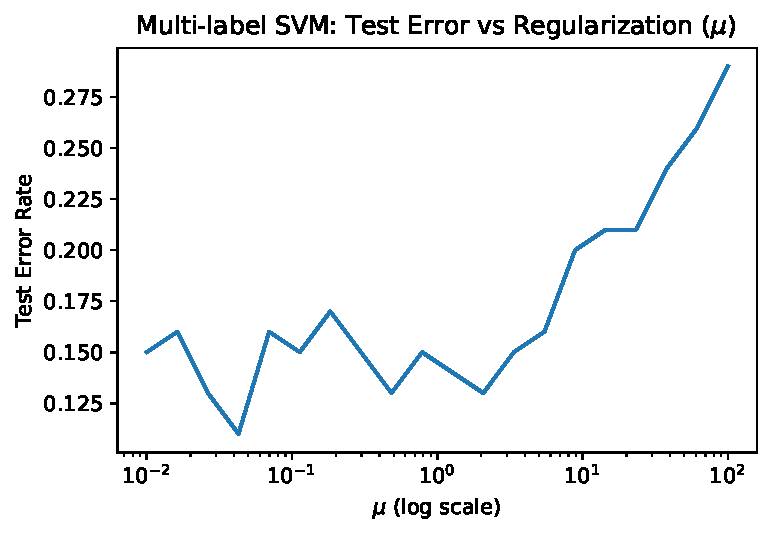
\includegraphics[keepaspectratio]{data_609_assignment_6_rerun_files/figure-pdf/cell-2-output-1.pdf}}

\subsection{Problem 2: Maximum Likelihood Prediction of Team Abilities
(Adapted from Exercise 7.4 in Convex Optimization Extended
Exercises)}\label{problem-2-maximum-likelihood-prediction-of-team-abilities-adapted-from-exercise-7.4-in-convex-optimization-extended-exercises}

A set of \(n\) teams compete in a tournament. We model each team's
ability by a number \(a_j,\, j = 1, \cdots , n\). When teams \(j\) and
\(k\) play each other, the probability that team \(j\) wins is equal to:

\[
\mathrm{prob}(a_j − a_k + v > 0)
\]

where \(v \sim \mathrm{Normal}(0, \sigma^2 )\). This means we can also
write the probability as
\(p(\mathrm{i\,\, beats \,\, j}) =  = \Phi\left(\frac{a_j-a_k}{\sigma}\right)\),
where \(\Phi\) is the cumulative distribution function of the standard
normal distribution.

You are given the outcome of \(m\) past games. These are organized as in
a game incidence matrix \(A\), where the \(l\)th row of \(A\)
corresponds to game \(l\) and where:

\[
A_{il} = \begin{cases} 1 \quad &\mathrm{if\,\,team\,\, i\,\, played\,\, in\,\, game\,\, l\,\, and\,\, won}  \\
-1 \quad &\mathrm{if\,\, team\,\, i\,\, played\,\, in\,\, game\,\, l\,\, and\,\, lost} l = k^{(i)} \\
0 \quad &\mathrm{otherwise}
\end{cases},
\]

This means that each row of \(A\) has exactly two non-zero entries, with
a \(1\) in the column of the team that played and won, and a \(-1\) in
the column of the team that played and lost.

\begin{enumerate}
\def\labelenumi{(\alph{enumi})}
\tightlist
\item
  Formulate the problem of finding the maximum likelihood estimate of
  team abilities, \(\hat{a} \in \mathbb{R}^n\), given the outcomes, as a
  convex optimization problem. Because the optimal solution can be
  shifted by a constant, you should specify a prior constraint on the
  first variable \(\hat{a}_0 = 0\).
\end{enumerate}

In order to keep the estimates bounded, an additional set of prior
constraints \(\hat{a}_i \in [-3, 3]\) should be included in the problem
formulation, and you should take \(\sigma = 0.25\) to be a constant
value rather than a variable. Also, we note that if a constant is added
to all team abilities, there is no change in the probabilities of game
outcomes.

This means that \(\hat{a}\) is determined only up to a constant, like a
potential. But this doesn't affect the ML estimation problem, or any
subsequent predictions made using the estimated parameters.

\begin{enumerate}
\def\labelenumi{(\alph{enumi})}
\setcounter{enumi}{1}
\tightlist
\item
  Find \(\hat{a}\) for the team data by the game incidence matrix
  \href{https://github.com/georgehagstrom/DATA609Spring2025/blob/main/website/assignments/labs/labData/AMat_train.csv}{AMat\_train.csv}.
  (This matrix gives the outcomes for a tournament in which each team
  plays each other team once.)
\end{enumerate}

You may find the CVX function \texttt{log\_normcdf} helpful for this
problem.

Remember that the cumulative distribution function of a log-concave
distribution is log-concave, and also that it is vectorized. Hint: the
\(l\)th row of \(A\mathrm{a} =a_{\mathrm{win},l}-a_{\mathrm{lose},l}\).

\begin{enumerate}
\def\labelenumi{(\alph{enumi})}
\setcounter{enumi}{2}
\tightlist
\item
  Use the maximum likelihood estimate \(\hat{a}\) found in part (b) to
  predict the outcomes of next year's tournament games, given in the
  file
  \href{https://github.com/georgehagstrom/DATA609Spring2025/blob/main/website/assignments/labs/labData/team_data_test.csv}{team\_data\_test.csv},
  using \[
  \hat{y}^{(i)} = \mathrm{sign}(\hat{a}_{j^{(i)}} − \hat{a}_{k^{(i)}})
  \]
\end{enumerate}

The first two rows of this file contain the indices of the two teams
playing, and the third column is \(1\) if the first team won and \(-1\)
otherwise. Compare the predictions predictions based on \(\hat{a}\) with
the actual outcomes, given in the third column of test. Give the
fraction of correctly predicted outcomes.

The games played in train and test are the same, so another, simpler
method for predicting the outcomes in test it to just assume the team
that won last year's match will also win this year's match. You can find
a similarly structured matrix in the file
\href{https://github.com/georgehagstrom/DATA609Spring2025/blob/main/website/assignments/labs/labData/team_data_test.csv}{team\_data\_test.csv},
or you can construct it from the game incidence matrix. Give the
percentage of correctly predicted outcomes using this simple method.

\subsubsection{Problem 2(a) Solution}\label{problem-2a-solution}

\[
\begin{aligned}
\max_{a \in \mathbb{R}^n} \quad & \sum_{l=1}^m \log\left( \Phi\left( \frac{(A a)_l}{0.25} \right) \right) \\
\text{subject to} \quad & a_0 = 0, \\
& a_i \in [-3, 3], \quad \forall i = 1, \dotsc, n.
\end{aligned}
\]

\subsubsection{Problem 2(b) and (c)
Solution}\label{problem-2b-and-c-solution}

\begin{Shaded}
\begin{Highlighting}[]
\CommentTok{\# load dependencies}
\ImportTok{import}\NormalTok{ numpy }\ImportTok{as}\NormalTok{ np}
\ImportTok{import}\NormalTok{ cvxpy }\ImportTok{as}\NormalTok{ cp}
\ImportTok{import}\NormalTok{ pandas }\ImportTok{as}\NormalTok{ pd}

\CommentTok{\# load data}
\NormalTok{train\_url }\OperatorTok{=} \StringTok{\textquotesingle{}https://media.githubusercontent.com/media/georgehagstrom/DATA609Spring2025/refs/heads/main/website/assignments/labs/labData/AMat\_train.csv\textquotesingle{}}
\NormalTok{A }\OperatorTok{=}\NormalTok{ pd.read\_csv(train\_url).values}

\CommentTok{\# define variables}
\NormalTok{m, n }\OperatorTok{=}\NormalTok{ A.shape}
\NormalTok{a }\OperatorTok{=}\NormalTok{ cp.Variable(n)}
\NormalTok{sigma }\OperatorTok{=} \FloatTok{0.25}

\CommentTok{\# define and calculate residual}
\NormalTok{residual }\OperatorTok{=}\NormalTok{ A }\OperatorTok{@}\NormalTok{ a}

\CommentTok{\# define the objective}
\NormalTok{objective }\OperatorTok{=}\NormalTok{ cp.}\BuiltInTok{sum}\NormalTok{(cp.log\_normcdf(residual }\OperatorTok{/}\NormalTok{ sigma))}

\CommentTok{\# define the constraint}
\NormalTok{constraints }\OperatorTok{=}\NormalTok{ [a[}\DecValTok{0}\NormalTok{] }\OperatorTok{==} \DecValTok{0}\NormalTok{, a }\OperatorTok{\textgreater{}=} \OperatorTok{{-}}\DecValTok{3}\NormalTok{, a }\OperatorTok{\textless{}=} \DecValTok{3}\NormalTok{]}

\CommentTok{\# define the problem}
\NormalTok{prob }\OperatorTok{=}\NormalTok{ cp.Problem(cp.Maximize(objective), constraints)}

\CommentTok{\# solve the problem}
\NormalTok{prob.solve(solver}\OperatorTok{=}\StringTok{\textquotesingle{}ECOS\textquotesingle{}}\NormalTok{, abstol}\OperatorTok{=}\FloatTok{1e{-}5}\NormalTok{, reltol}\OperatorTok{=}\FloatTok{1e{-}5}\NormalTok{, max\_iters}\OperatorTok{=}\DecValTok{10000}\NormalTok{)}

\CommentTok{\# print result}
\NormalTok{ahat }\OperatorTok{=}\NormalTok{ a.value}
\BuiltInTok{print}\NormalTok{(}\StringTok{"}\CharTok{\textbackslash{}n}\StringTok{Estimated team abilities (ahat):}\CharTok{\textbackslash{}n}\StringTok{"}\NormalTok{, ahat)}

\CommentTok{\# load the test data}
\NormalTok{test\_data\_url }\OperatorTok{=} \StringTok{\textquotesingle{}https://media.githubusercontent.com/media/georgehagstrom/DATA609Spring2025/refs/heads/main/website/assignments/labs/labData/team\_data\_test.csv\textquotesingle{}}
\NormalTok{test\_data }\OperatorTok{=}\NormalTok{ pd.read\_csv(test\_data\_url).values}

\CommentTok{\# split the test data into team 1 and team 2}
\NormalTok{team1\_indices }\OperatorTok{=}\NormalTok{ test\_data[:, }\DecValTok{0}\NormalTok{].astype(}\BuiltInTok{int}\NormalTok{)  }
\NormalTok{team2\_indices }\OperatorTok{=}\NormalTok{ test\_data[:, }\DecValTok{1}\NormalTok{].astype(}\BuiltInTok{int}\NormalTok{)  }
\NormalTok{actual\_outcomes }\OperatorTok{=}\NormalTok{ test\_data[:, }\DecValTok{2}\NormalTok{]            }

\CommentTok{\# calculate the predicted value based on a\_hat}

\NormalTok{predictions }\OperatorTok{=}\NormalTok{ np.sign(ahat[team1\_indices] }\OperatorTok{{-}}\NormalTok{ ahat[team2\_indices])}

\CommentTok{\# define and calculate accuracy}
\NormalTok{correct }\OperatorTok{=}\NormalTok{ np.}\BuiltInTok{sum}\NormalTok{(predictions }\OperatorTok{==}\NormalTok{ actual\_outcomes)}
\NormalTok{total }\OperatorTok{=} \BuiltInTok{len}\NormalTok{(actual\_outcomes)}
\NormalTok{accuracy }\OperatorTok{=}\NormalTok{ correct }\OperatorTok{/}\NormalTok{ total}

\CommentTok{\# apply the prediction}
\NormalTok{last\_year\_winners }\OperatorTok{=}\NormalTok{ np.argmax(A }\OperatorTok{==} \DecValTok{1}\NormalTok{, axis}\OperatorTok{=}\DecValTok{1}\NormalTok{)}
\NormalTok{last\_year\_losers }\OperatorTok{=}\NormalTok{ np.argmax(A }\OperatorTok{==} \OperatorTok{{-}}\DecValTok{1}\NormalTok{, axis}\OperatorTok{=}\DecValTok{1}\NormalTok{)}
\NormalTok{simple\_predictions }\OperatorTok{=}\NormalTok{ np.where(}
\NormalTok{    team1\_indices }\OperatorTok{==}\NormalTok{ last\_year\_winners, }\DecValTok{1}\NormalTok{,}
\NormalTok{    np.where(team2\_indices }\OperatorTok{==}\NormalTok{ last\_year\_winners, }\OperatorTok{{-}}\DecValTok{1}\NormalTok{, }\DecValTok{0}\NormalTok{)}
\NormalTok{)}

\CommentTok{\# compare the predicted value with the actual outcome}
\NormalTok{correct\_simple }\OperatorTok{=}\NormalTok{ np.}\BuiltInTok{sum}\NormalTok{(simple\_predictions }\OperatorTok{==}\NormalTok{ actual\_outcomes)}
\NormalTok{accuracy\_simple }\OperatorTok{=}\NormalTok{ correct\_simple }\OperatorTok{/}\NormalTok{ total}

\BuiltInTok{print}\NormalTok{(}\SpecialStringTok{f"}\CharTok{\textbackslash{}n}\SpecialStringTok{Prediction accuracy assuming last year\textquotesingle{}s winner wins again: }\SpecialCharTok{\{}\NormalTok{accuracy\_simple}\SpecialCharTok{:.4f\}}\SpecialStringTok{ (}\SpecialCharTok{\{}\NormalTok{accuracy\_simple}\OperatorTok{*}\DecValTok{100}\SpecialCharTok{:.2f\}}\SpecialStringTok{\%)"}\NormalTok{)}
\end{Highlighting}
\end{Shaded}

\begin{verbatim}

Estimated team abilities (ahat):
 [-8.36354694e-11  2.90412993e+00 -1.12088515e+00  1.82166813e+00
 -2.00997238e+00  1.99242627e+00  1.98096517e+00  5.89411388e-01
 -2.92179720e+00  1.81020704e+00 -2.82541274e-01]

Prediction accuracy assuming last year's winner wins again: 0.9778 (97.78%)
\end{verbatim}

\subsection{Problem 3: Flux balance analysis in systems biology.
(Exercise 21.3 in CVX Additional
Exercises)}\label{problem-3-flux-balance-analysis-in-systems-biology.-exercise-21.3-in-cvx-additional-exercises}

Flux balance analysis is based on a very simple model of the reactions
going on in a cell, keeping track only of the gross rate of consumption
and production of various chemical species within the cell. Based on the
known stoichiometry of the reactions, and known upper bounds on some of
the reaction rates, we can compute bounds on the other reaction rates,
or cell growth, for example.

We focus on \(m\) metabolites in a cell, labeled \(M_1\) , . . . ,
\(M_m\) . There are \(n\) reactions going on, labeled \(R_1\) , . . . ,
\(R_n\) , with nonnegative reaction rates \(v_1\) , . . . , \(v_n\).

In our particular case, we will be working with a simplified model of
cell metabolism having 9 reactions and 6 metabolites. Each reaction has
a (known) stoichiometry, which tells us the rate of consumption and
production of the metabolites per unit of reaction rate.

The stoichiometry data is given by the stoichiometry matrix
\(S \in \mathbb{R}^{m\times n}\) , defined as follows: \(S_{ij}\) is the
rate of production of \(M_i\) due to unit reaction rate \(v_j = 1\).

Here we consider consumption of a metabolite as negative production; so
\(S_{ij} = −2\), for example, means that reaction \(\mathbb{R}^j\)
causes metabolite \(M_i\) to be consumed at a rate \(2v_j\) .

As an example, suppose reaction \(R_1\) has the form
\(M_1 \to M_2 + 2M_3\) . The consumption rate of \(M_1\) , due to this
reaction, is \(v_1\) ; the production rate of \(M_2\) is \(v_1\) ; and
the production rate of \(M_3\) is \(2v_1\) . (The reaction \(R_1\) has
no effect on metabolites \(M_4\) , . . . , \(M_m\) .)

This corresponds to a first column of \(S\) of the form
\((−1, 1, 2, 0, \dots , 0)\).

Reactions are also used to model flow of metabolites into and out of the
cell. For example, suppose that reaction \(R_2\) corresponds to the flow
of metabolite \(M_1\) into the cell, with \(v_2\) giving the flow rate.
This corresponds to a second column of \(S\) of the form
\((1, 0, . . . , 0)\).

The last reaction, \(R_n\) , corresponds to biomass creation, or cell
growth, so the reaction rate \(v_n\) is the cell growth rate. The last
column of \(S\) gives the amounts of metabolites used or created per
unit of cell growth rate.

Since our reactions include metabolites entering or leaving the cell, as
well as those converted to biomass within the cell, we have conservation
of the metabolites, which can be expressed as \(Sv = 0\). In addition,
we are given upper limits on some of the reaction rates, which we
express as \(v \preceq v^{\mathrm{max}}\) , where we set
\(v_{j}^{\mathrm{max}} = \infty\) if no upper limit on reaction rate
\(j\) is known.

The goal is to find the maximum possible cell growth rate (i.e., largest
possible value of \(v_n\) ) consistent with the constraints:

\[
\mathrm{max}_v v_9 \\
Sv = 0 \\
v \succeq 0 \\
v \preceq v^{\mathrm{max}} 
\]

The questions below pertain to the data found in
\href{https://github.com/georgehagstrom/DATA609Spring2025/blob/main/website/assignments/labs/labData/fba_S.csv}{fba\_S.csv}
and
\href{https://github.com/georgehagstrom/DATA609Spring2025/blob/main/website/assignments/labs/labData/fba_vmax.csv}{fba\_vmax.csv},
which contain the Stoichiometric Matrix and the upper bounds on the
reaction fluxes, respectively. This exercise was inspired by the
following paper:
\href{https://www.liebertpub.com/doi/abs/10.1089/153623103322452413}{Segre
et all 2003}

\begin{enumerate}
\def\labelenumi{(\alph{enumi})}
\item
  Find the maximum possible cell growth rate \(G^{\star}\) , as well as
  optimal Lagrange multipliers for the reaction rate limits. How
  sensitive is the maximum growth rate to the various reaction rate
  limits?
\item
  Essential genes and synthetic lethals. For simplicity, we'll assume
  that each reaction is controlled by an associated gene, i.e., gene
  \(G_i\) controls reaction \(R_i\) .
\end{enumerate}

Knocking out a set of genes associated with some reactions has the
effect of setting the reaction rates (or equivalently, the associated v
max entries) to zero, which of course reduces the maximum possible
growth rate.

If the maximum growth rate becomes small enough or zero, it is
reasonable to guess that knocking out the set of genes will kill the
cell. An essential gene is one that when knocked out reduces the maximum
growth rate below a given threshold \(G^{\mathrm{min}}\) . (Note that
\(G_n\) is always an essential gene.)

A synthetic lethal is a pair of non-essential genes that when knocked
out reduces the maximum growth rate below the threshold. Find all
essential genes and synthetic lethals for the given problem instance,
using the threshold \(G^{\mathrm{min}} = 0.2G^{\star}\) .

\subsubsection{Problem 3(a) and (b)
Solution}\label{problem-3a-and-b-solution}

\begin{Shaded}
\begin{Highlighting}[]
\CommentTok{\# load dependencies}
\ImportTok{import}\NormalTok{ numpy }\ImportTok{as}\NormalTok{ np}
\ImportTok{import}\NormalTok{ pandas }\ImportTok{as}\NormalTok{ pd}
\ImportTok{from}\NormalTok{ scipy.optimize }\ImportTok{import}\NormalTok{ linprog}
\ImportTok{from}\NormalTok{ itertools }\ImportTok{import}\NormalTok{ combinations}

\CommentTok{\# load data}
\NormalTok{fba\_s\_url }\OperatorTok{=} \StringTok{\textquotesingle{}https://media.githubusercontent.com/media/georgehagstrom/DATA609Spring2025/refs/heads/main/website/assignments/labs/labData/fba\_S.csv\textquotesingle{}}
\NormalTok{fba\_vmax\_url }\OperatorTok{=} \StringTok{\textquotesingle{}https://media.githubusercontent.com/media/georgehagstrom/DATA609Spring2025/refs/heads/main/website/assignments/labs/labData/fba\_vmax.csv\textquotesingle{}}

\CommentTok{\# define the data}
\NormalTok{S }\OperatorTok{=}\NormalTok{ pd.read\_csv(fba\_s\_url, index\_col }\OperatorTok{=} \DecValTok{0}\NormalTok{).values}
\NormalTok{vmax }\OperatorTok{=}\NormalTok{ pd.read\_csv(fba\_vmax\_url, index\_col}\OperatorTok{=} \DecValTok{0}\NormalTok{).values.flatten()}
\NormalTok{S }\OperatorTok{=}\NormalTok{ np.array(S, dtype}\OperatorTok{=}\BuiltInTok{float}\NormalTok{).T}
\NormalTok{vmax }\OperatorTok{=}\NormalTok{ np.array(vmax, dtype}\OperatorTok{=}\BuiltInTok{float}\NormalTok{)}

\CommentTok{\# define variables}
\NormalTok{c }\OperatorTok{=}\NormalTok{ np.zeros(}\DecValTok{9}\NormalTok{)}
\NormalTok{c[}\DecValTok{8}\NormalTok{] }\OperatorTok{=} \OperatorTok{{-}}\DecValTok{1}  
\NormalTok{A\_eq }\OperatorTok{=}\NormalTok{ S}
\NormalTok{b\_eq }\OperatorTok{=}\NormalTok{ np.zeros(S.shape[}\DecValTok{0}\NormalTok{])}
\NormalTok{bounds }\OperatorTok{=}\NormalTok{ [(}\DecValTok{0}\NormalTok{, vmax[i]) }\ControlFlowTok{for}\NormalTok{ i }\KeywordTok{in} \BuiltInTok{range}\NormalTok{(}\DecValTok{9}\NormalTok{)]}

\CommentTok{\# define and solve the max growth}
\NormalTok{res }\OperatorTok{=}\NormalTok{ linprog(c, A\_eq}\OperatorTok{=}\NormalTok{A\_eq, b\_eq}\OperatorTok{=}\NormalTok{b\_eq, bounds}\OperatorTok{=}\NormalTok{bounds, method}\OperatorTok{=}\StringTok{\textquotesingle{}highs\textquotesingle{}}\NormalTok{)}
\NormalTok{G\_star }\OperatorTok{=}\NormalTok{ res.x[}\DecValTok{8}\NormalTok{]}

\CommentTok{\# define the duality of essential and nonessential}

\NormalTok{dual\_vmax }\OperatorTok{=}\NormalTok{ res.upper}
\NormalTok{G\_min }\OperatorTok{=} \FloatTok{0.2} \OperatorTok{*}\NormalTok{ G\_star}
\NormalTok{essential }\OperatorTok{=}\NormalTok{ []}
\ControlFlowTok{for}\NormalTok{ i }\KeywordTok{in} \BuiltInTok{range}\NormalTok{(}\DecValTok{9}\NormalTok{):}
\NormalTok{    vmax\_ko }\OperatorTok{=}\NormalTok{ vmax.copy()}
\NormalTok{    vmax\_ko[i] }\OperatorTok{=} \DecValTok{0}
\NormalTok{    bounds\_ko }\OperatorTok{=}\NormalTok{ [(}\DecValTok{0}\NormalTok{, vmax\_ko[j]) }\ControlFlowTok{for}\NormalTok{ j }\KeywordTok{in} \BuiltInTok{range}\NormalTok{(}\DecValTok{9}\NormalTok{)]}
\NormalTok{    res\_ko }\OperatorTok{=}\NormalTok{ linprog(c, A\_eq}\OperatorTok{=}\NormalTok{A\_eq, b\_eq}\OperatorTok{=}\NormalTok{b\_eq, bounds}\OperatorTok{=}\NormalTok{bounds\_ko, method}\OperatorTok{=}\StringTok{\textquotesingle{}highs\textquotesingle{}}\NormalTok{)}
    \ControlFlowTok{if} \KeywordTok{not}\NormalTok{ res\_ko.success }\KeywordTok{or}\NormalTok{ res\_ko.x[}\DecValTok{8}\NormalTok{] }\OperatorTok{\textless{}}\NormalTok{ G\_min:}
\NormalTok{        essential.append(i}\OperatorTok{+}\DecValTok{1}\NormalTok{)}

\NormalTok{nonessential }\OperatorTok{=}\NormalTok{ [i }\ControlFlowTok{for}\NormalTok{ i }\KeywordTok{in} \BuiltInTok{range}\NormalTok{(}\DecValTok{9}\NormalTok{) }\ControlFlowTok{if}\NormalTok{ (i}\OperatorTok{+}\DecValTok{1}\NormalTok{) }\KeywordTok{not} \KeywordTok{in}\NormalTok{ essential]}
\NormalTok{synthetic }\OperatorTok{=}\NormalTok{ []}
\ControlFlowTok{for}\NormalTok{ i, j }\KeywordTok{in}\NormalTok{ combinations(nonessential, }\DecValTok{2}\NormalTok{):}
\NormalTok{    vmax\_ko }\OperatorTok{=}\NormalTok{ vmax.copy()}
\NormalTok{    vmax\_ko[i] }\OperatorTok{=}\NormalTok{ vmax\_ko[j] }\OperatorTok{=} \DecValTok{0}
\NormalTok{    bounds\_ko }\OperatorTok{=}\NormalTok{ [(}\DecValTok{0}\NormalTok{, vmax\_ko[k]) }\ControlFlowTok{for}\NormalTok{ k }\KeywordTok{in} \BuiltInTok{range}\NormalTok{(}\DecValTok{9}\NormalTok{)]}
\NormalTok{    res\_ko }\OperatorTok{=}\NormalTok{ linprog(c, A\_eq}\OperatorTok{=}\NormalTok{A\_eq, b\_eq}\OperatorTok{=}\NormalTok{b\_eq, bounds}\OperatorTok{=}\NormalTok{bounds\_ko, method}\OperatorTok{=}\StringTok{\textquotesingle{}highs\textquotesingle{}}\NormalTok{)}
    \ControlFlowTok{if} \KeywordTok{not}\NormalTok{ res\_ko.success }\KeywordTok{or}\NormalTok{ res\_ko.x[}\DecValTok{8}\NormalTok{] }\OperatorTok{\textless{}}\NormalTok{ G\_min:}
\NormalTok{        synthetic.append((i}\OperatorTok{+}\DecValTok{1}\NormalTok{, j}\OperatorTok{+}\DecValTok{1}\NormalTok{))}

\CommentTok{\# print result}
\BuiltInTok{print}\NormalTok{(}\SpecialStringTok{f"Maximum growth rate G* = }\SpecialCharTok{\{}\NormalTok{G\_star}\SpecialCharTok{:.4f\}}\SpecialStringTok{"}\NormalTok{)}
\BuiltInTok{print}\NormalTok{(}\StringTok{"Essential genes (reactions):"}\NormalTok{, essential)}
\BuiltInTok{print}\NormalTok{(}\StringTok{"Synthetic lethal pairs:"}\NormalTok{, synthetic)}
\BuiltInTok{print}\NormalTok{(}\StringTok{"Dual values for reaction bounds:"}\NormalTok{, dual\_vmax)}
\end{Highlighting}
\end{Shaded}

\begin{verbatim}
Maximum growth rate G* = 13.5500
Essential genes (reactions): [1, 9]
Synthetic lethal pairs: [(2, 3), (2, 7), (4, 7), (5, 7)]
Dual values for reaction bounds:  marginals: array([-0.5,  0. , -0.5,  0. , -1.5,  0. ,  0. ,  0. ,  0. ])
  residual: array([ 0.  , 95.8 ,  0.  , 96.3 ,  0.  , 99.75, 93.85, 99.75, 86.45])
\end{verbatim}




\end{document}
